%\documentclass[notes,10pt,aspectratio=169]{beamer}

%\documentclass[notes, 10pt,aspectratio=169]{beamer}
\documentclass[10pt,aspectratio=169]{beamer}


% Add this line to your preamble
\setbeameroption{show notes on second screen=right}

%\usetheme{Singapore} %Boadilla, Madrid, default, etc. 
\usetheme[progressbar=frametitle]{metropolis}
\usecolortheme{rose} %beaver, dolphin, crane, 


%\setbeamersize{text margin left=4mm, text margin right=4mm}


\usecolortheme{default}

\usepackage[utf8]{inputenc}
\usepackage[T1]{fontenc}
\usepackage{lmodern}
\usepackage{xcolor}
\usepackage{tikz}
\usepackage{booktabs} % Required for \toprule, \midrule, \bottomrule
\usetikzlibrary{shapes.geometric, arrows, positioning}

\tikzstyle{block} = [rectangle, draw, text width=4cm, align=center, rounded corners, minimum height=1cm]
\tikzstyle{decision} = [rectangle, draw, text width=5cm, align=center, fill=blue!10, rounded corners, minimum height=1cm]
\tikzstyle{terminal} = [rectangle, draw, text width=4.5cm, align=center, fill=yellow!30, rounded corners, minimum height=1cm]
\tikzstyle{end} = [rectangle, draw, text width=5cm, align=center, fill=green!30, rounded corners, minimum height=1cm]
\tikzstyle{arrow} = [->, thick]



\usepackage{adjustbox}
%2. change the bullets 
\setbeamertemplate{itemize item}[triangle] %circle, square,... 


% 1. Define custom colors and set colors 
%\definecolor{myblue}{HTML}{003366}
\definecolor{accent}{RGB}{78,205,196}

%\setbeamercolor{title}{fg=white,bg=myblue}
\setbeamercolor{frametitle}{fg=black,bg=white}
%\setbeamercolor{normal text}{fg=mygray}
\setbeamercolor{block title}{fg=black,bg=blue}
%\setbeamercolor{block body}{fg=black,bg=white}

\setbeamercolor{item}{fg= orange!80} % Change bullet color
\setbeamercolor{button}{bg=orange, fg=white}





% 3. BibLaTeX settings
\usepackage[
  backend=biber,
  style=apa,
  citestyle=authoryear
]{biblatex}
\addbibresource{references.bib}

\title{Aftermarkets: Evidence from a Centralized Annuities marketplace}
%\subtitle{A Mini Literature Overview}

\author{%
 Lucas Condeza
\inst{1} \and
   %\and
%  Coauthor Three\inst{3}
}
\institute{
  \inst{1} Yale University \\
}

\date{\today}

\begin{document}

\begin{frame}
  \titlepage
\end{frame}



 %%%%%%%%%

\begin{frame}{Research question}
    
\begin{itemize}
    
    \item \textbf{What is the impact of Aftermarkets?}

    \begin{itemize}
    \item  What are \textit{Aftermarkets}? 
    \item Some examples 
    \item What are annuities? and  their price 
    \item Setting 
    \end{itemize}
 \textcolor{red}{[Is the question interesting? ]}\textcolor{red}{[Is aftermarket  the correct term? ]}
 
\end{itemize}

\note{\scriptsize %\footnotesize
Instead of a dedicated “Feedback” slide, I will annotate my slides in red with the questions I’d like feedback on.

My research question is what are the impacts of aftermarkets?.  First I will define what I mean by an aftermarket, secondly I will provide some examples and third mention the setting where I plan to study it. 

1. In many digital marketplaces sellers first post an initial price. After observing the price buyers can buy from one of the sellers or request a revised price, I will refer to this as search. I will refer to this second stage where a consumer asks for a revised price as the aftermarket. There are three important aspects about the revised prices, 1)they can be costly to request,  2) I am using request in a broad sense, it could mean that the buyer bargains with the seller or  the seller posts a revised price and 3) they might involve some face to face interaction.  

2. For example in Zillow, which is a marketplace for buying houses, sellers post an initial price, but the buyer can bargain with the seller to get a discount over the initial price. This feature is also present in other marketplaces like Autotrader, which is a marketplace to buy cars. 

3. An annuity is a financial contract where, in exchange for a lump-sum payment, an insurer guarantees a fixed payment each period thereafter. I will refer to the price of an annuity to the price of buying a contract that pays 1\$ each period.

4. The setting I plan to study is a centralized annuities market in Chile. Insurers- who sell the annuities- post an initial buyer-specific price, then the buyer either buys from one of the insurers or requests a revised price from one of the insurers who posted a price. A recently passed law banned the aftermarket, because according to policymakers it reduced incentives for firms to post low prices in the initial stage. 
}

\end{frame}
%%%%%%%%%

\begin{frame}\frametitle{Different use of the aftermarket}\label{slide:single_fig}
\begin{figure}
    \centering
    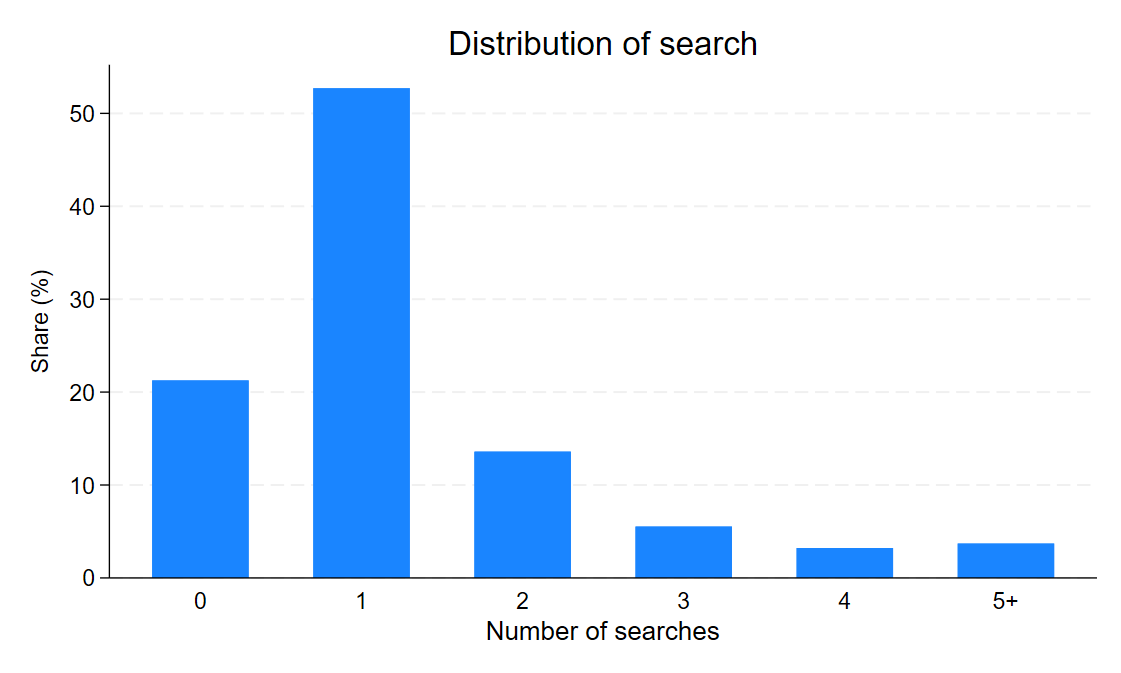
\includegraphics[width=0.49\textwidth]{../figures/IE3_dist_external_offers.png}
    \hfill 
    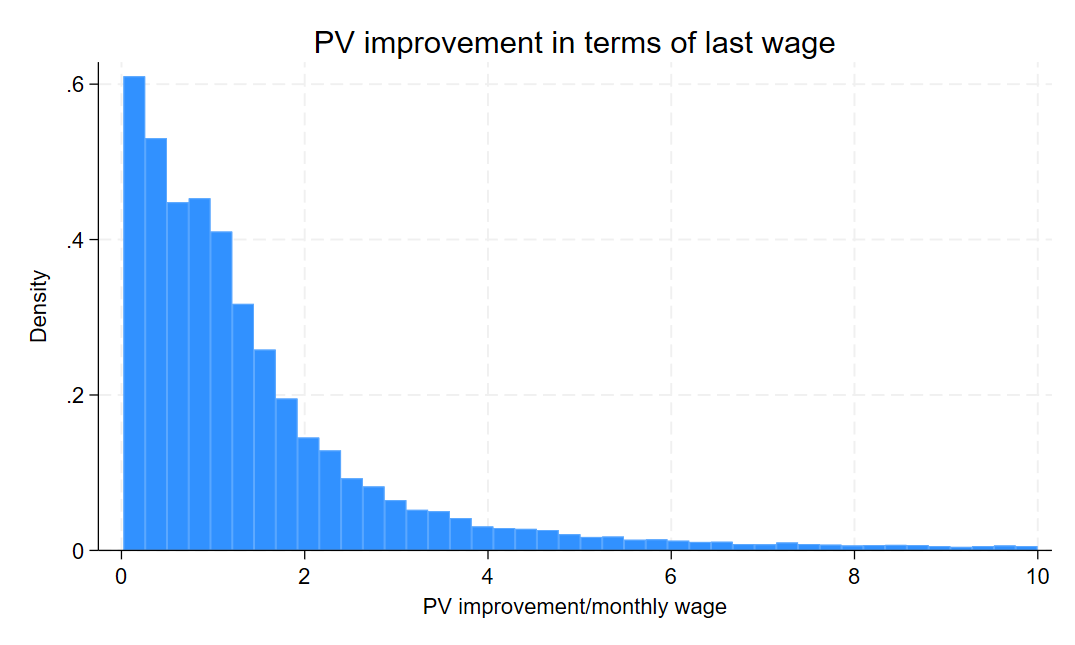
\includegraphics[width=0.49\textwidth]{../figures/IE3_offer_improvement_histogram.png}
\end{figure}

\begin{itemize}
    \item   75\% of the purchases are through the aftermarket 
     \hyperlink{slide:fig4}{\beamerbutton{Search by income}} 
    
    \textcolor{red}{[What are the determinants of search? Search direction?] }
\end{itemize}

\note{
That only some people use the aftermarket suggest: 
\begin{itemize}
    \item There are search costs 
    \item Firms could be discriminating based on the search likelihood. 
\end{itemize}
Any assessment of the welfare effects of the aftermarket has to consider that by banning it buyers will save in search costs, but will not be able to improve on the initial posted prices. 

In a model where search costs are not correlated with valuations, the aftermarket prices by the sellers are the same as the initial prices.
}
\end{frame}

%%%%%%%%%%%%%%%%%%%%%%%%%

\begin{frame}{Literature}
\begin{itemize}
    \item Aftermarkets: \textcite{larsen_efficiency_2021, allen_search_2019}

    \item Competition in selection markets: \textcite{mahoney_imperfect_2017, cuesta_price_2018, cosconati_competing_2025}

    \item Selection in multiple dimensions: \textcite{finkelstein_adverse_2004} and Finkelstein and McGarry (2006).  
\end{itemize}
\end{frame}

%%%%%%%%%%%%%%%%%%%%%%%%%
 
\begin{frame}{Annuities in Chile: SCOMP}  \label{slide:setting}
       
    \begin{itemize}%[<+->]
    \item SCOMP steps: 
    \begin{enumerate}
        \item Request of balance statement 
        \item Request for offers: asks for certain type of contracts (e.g. annuity)
        \item Insurers post initial prices (e.g. \$20 per \$1 of flow) \hyperlink{slide:fig5}{\beamerbutton{Offer Certificate}}
        \item Retiree chooses one of the insurers or asks for revised prices

    \end{enumerate}

        \item Revised prices: bargaining and information disclosure
        

    \item Firms competition 1. financing cost 2. prediction algorithm 

    \item Profits of firm $j$: 
    \begin{align*}
    \pi_{ji}(F) = S_i-  \mathbb{E}^j_{T} \left[\sum_{t=1}^T\frac{F}{(1+r_j)^t}|x_i \right]
    \end{align*}
    % if it was only financing cost, it would be a monopoly
    \end{itemize}

     $S$: stock of savings, $F$: per period annuity payment, $x_i$: individual mortality factors
    \textcolor{red}{[In what dimensions do insurers differ? ]}
    \note{
    \begin{itemize}
        \item Explicitly not link the annuities market with pensions because generates confusion
        \item Explain what annuities are. 
    \end{itemize}}
\end{frame}

%%%%%%%%%%%%%%%%%%%%%%%%%%%%%%%%%%%%%%

 \begin{frame}{Data} \label{slide:data}
\begin{itemize}
    \item SCOMP data at the individual level  
    \begin{itemize}
        \item Posted and revised prices, and consumer decisions 
        \item Total savings 
        \item Demographics: age and gender \hyperlink{slide:fig5}{\beamerbutton{Certificate with initial prices}}
    \end{itemize}
     \item Retirement insurance companies: risk ratings
\end{itemize}
\note{Important to mention that the advantage of our data is that 1) elicits prices from almost all companies and 2) records all the elicited prices. }
\end{frame}

%%%%%%%%%%%%%%%%%%%%%%%
\begin{frame}{Answer the question}\label{slide:answer1}
    \begin{itemize}
        \item Equilibrium model of search and revised prices  
        \begin{itemize}
            \item First stage: sellers post initial prices and consumers buy or search 
            \item Second stage: If buyer searches is matched with a seller and they bargain
        \end{itemize}
        \item Desiderata:
        \begin{itemize}
           \item Imperfect-assymmetric competition\hyperlink{slide:fig2}{\beamerbutton{Evidence}}
            \item Differentiated products   \hyperlink{slide:fig3}{\beamerbutton{Evidence}}
            \item Adverse selection
        \end{itemize}
    \end{itemize}

    \textcolor{red}{[How to model selection with competition?]}
    \note{\textbf{ Imperfect-assymmetric competition:} the differences in market share can be due to preferences, but not so the differences in probability of posting a price
   
   \textbf{Diff products:} if not the case then everyone would choose the lowest price
   }
\end{frame}


%%%%%%%%%%%%%%%%%%%%%


\begin{frame}{Firm specialization}\label{slide:fig1}    

Firm specialization in groups
\begin{figure}[H]
%\caption{}
\centering{}%
\begin{tabular}{cc}
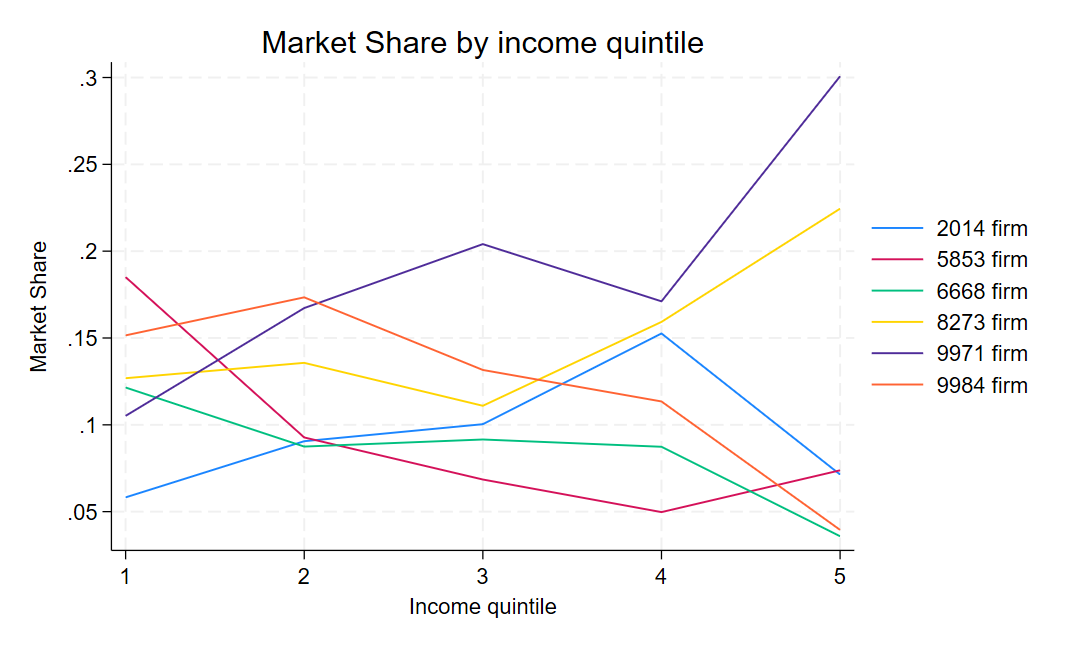
\includegraphics[scale=0.27]{../figures/IE3_supply_income_quintile.png}
\end{tabular}
\end{figure}

\hyperlink{slide:answer1}{\beamerbutton{Go back}}

\end{frame}

%%%%%%%%%%%%%%%%%%%%%

\begin{frame}{Firm specialization(2)}\label{slide:fig2}    

\begin{figure}[H]
\caption{}
\centering{}%
\begin{tabular}{cc}
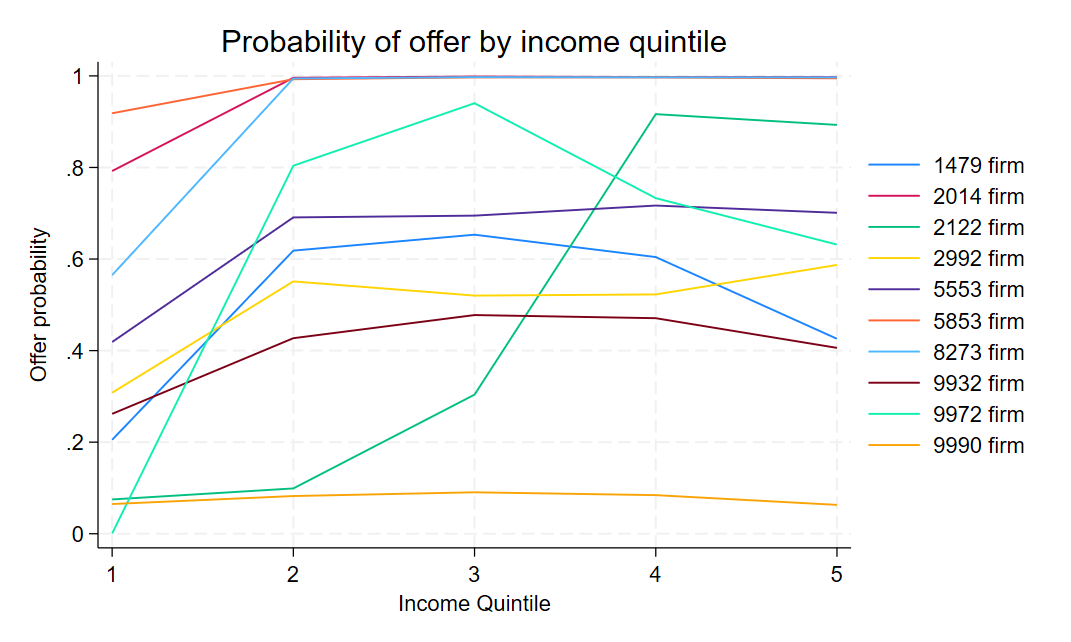
\includegraphics[scale=0.24]{../figures/IE3_supply_offerprob_income_q(2).png}
\end{tabular}
\end{figure}

Firms specialize on buyer types
\hyperlink{slide:answer1}{\beamerbutton{Go back}}

\end{frame}

%%%%%%%%%%%%%%%%%%%%%

\begin{frame}{Heterogeneity in preferences}\label{slide:fig3}    

Buyers do not always buy highest annuity. Average foregone value is 1.57 monthly wages.

\begin{figure}[H]
%\caption{}
\centering{}%
\begin{tabular}{cc}
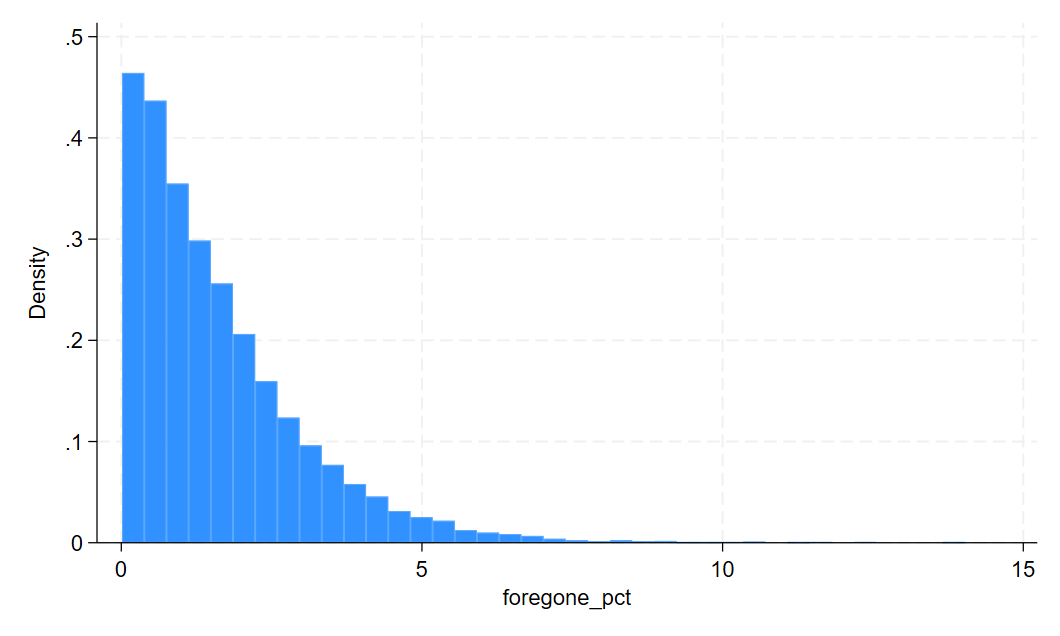
\includegraphics[scale=0.25]{../figures/IE3_foregone_hist.png}
\end{tabular}
\end{figure}
\hyperlink{slide:answer1}{\beamerbutton{Go back}}

\end{frame}

%%%%%%%%%%%%%%%%%%%%%

\begin{frame}{Search(2)}\label{slide:fig4}    

\begin{figure}[H]
%\caption{}
\centering{}%
\begin{tabular}{cc}
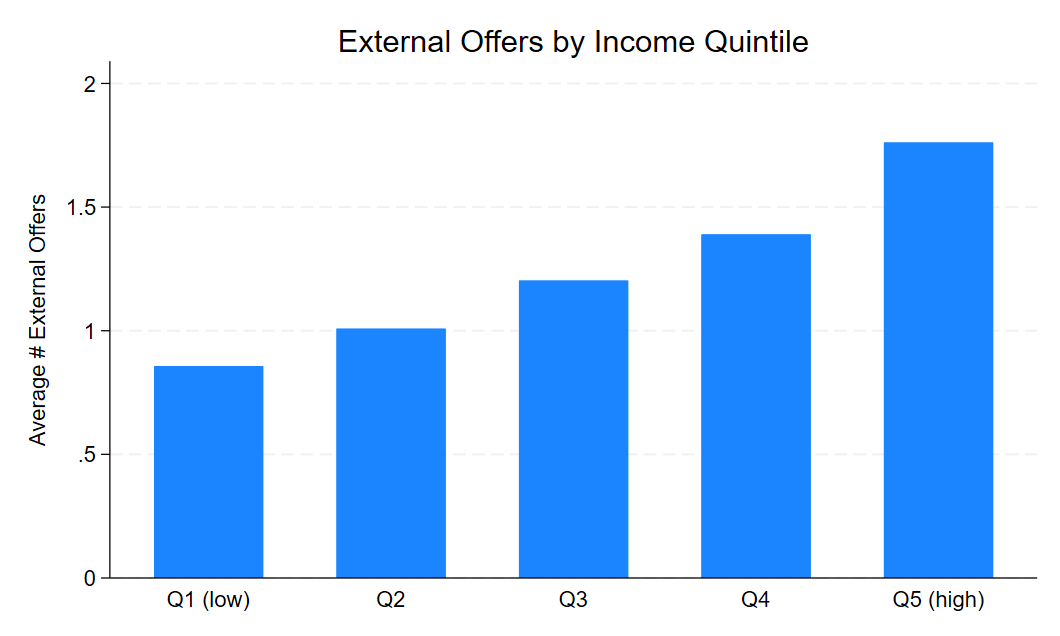
\includegraphics[scale=0.27]{../figures/IE3_search_by_income_quintile.png}
\end{tabular}
\end{figure}
\hyperlink{slide:single_fig}{\beamerbutton{Go back}}
\end{frame}

\begin{frame}{Initial prices}\label{slide:fig5}    
\begin{figure}[H]
%\caption{}
\centering{}%
\begin{tabular}{cc}
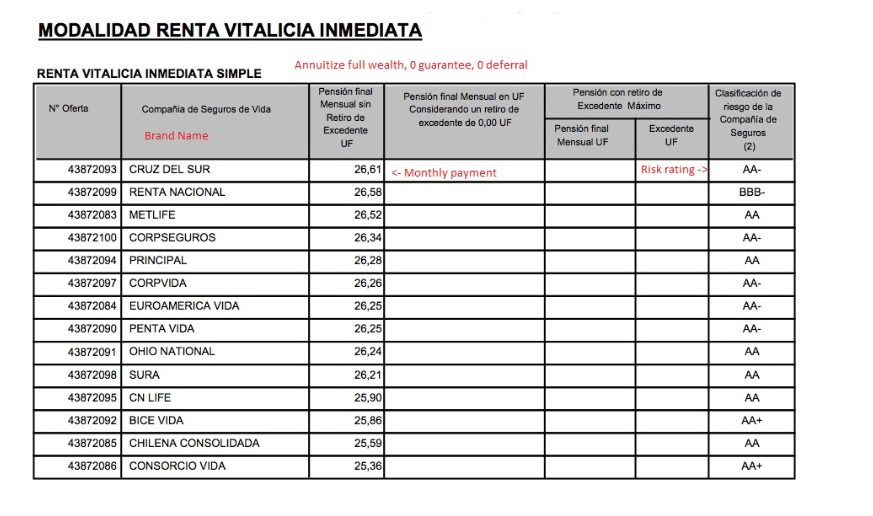
\includegraphics[scale=0.49]{../figures/annuity_offer.png}
\end{tabular}
\end{figure}
\hyperlink{slide:setting}{\beamerbutton{Go back}}
\end{frame}


\end{document}